\nsection{OSN 14 Спецификация и верификация параллельных программ. Синхронная и асинхронная параллельность. Справедливость планировщика.Темпоральная логика линейного времени (LTL). Проблема взаимного исключения процессов.}

1) смотри сюда: \url{http://sp.cmc.msu.ru/courses/vmp/kamkin_mc2018.pdf}, 
Страничка 135

Рассмотрим следующую упрощенную модель.
\textbf{Параллельной программой} \textit{P}, или просто программой, называется конечное множество последовательных программ \textit{$P_i$} над общим множеством переменных. 
Отдельная программа этого множества называется \textit{процессом}.
Переменные, используемые только в одном процессе, называются \textit{локальными}; переменные, используемые в нескольких процессах, — \textit{разделяемыми} или \textit{глобальными}.
\textit{Семантика}, или \textit{модель вычислений}, параллельной программы может быть определена, используя парадигму \textit{чередования} (интерливинга), известную также как \textbf{асинхронный параллелизм}. 
\textit{Стратегию} выбора процесса, также как и сущность, реализующую эту стратегию, мы будем называть \textbf{планировщиком}. 

При анализе свойств реагирующих систем предполагают, что \textit{планировщик} является \textbf{справедливым}, т.е. каждый процесс периодически, время от времени, выбирается для исполнения; другими словами, невозможна ситуация, когда какой-нибудь процесс не выбирается бесконечно долго.

Такая модель вычислений, известная как \textbf{синхронный параллелизм}, широко используется при проектировании цифровой аппаратуры. 
В этой модели параллельные присваивания в одну переменную либо запрещаются, либо совершается только одно из них, выбранное \textit{недетерминированным образом}.

Далее мы будем рассматривать исключительно \textit{асинхронные} параллельные программы. 
Более того, мы будем рассматривать программы, работающие в «бесконечном цикле». 
Речь идет о так называемых \textit{реагирующих}, или \textit{реактивных}, системах (от англ. reactive). 
Такие системы реагируют на события окружения, выполняя в ответ те или иные действия. 
Это обширный класс программ, включающий операционные системы, драйверы устройств, телекоммуникационные среды, системы управления и т.п.
На данном этапе под \textit{событием} понимается условие на значения разделяемых переменных (\textit{охранное условие}, или \textit{защита}), а под \textit{действием} — часть программы, срабатывающая, когда условие становится истинным. 


\paragraph{\textbf{Темпоральная логика} линейного времени (LTL, Linear-time Temporal Logic).} 
\text{}
\newline
В LTL к синтаксису классической логики высказываний добавлены два темпоральных оператора: унарный оператор \textbf{X} (от англ. ne\textbf{X}t time — в следующий момент времени) и бинарный оператор \textbf{U} (от англ. \textbf{U}ntil — до тех пор, пока не). 
Эти два оператора образуют \textbf{темпоральный базис LTL}. 
Формула логики LTL задается следующей грамматикой:
\begin{equation}
  \phi ::= p | \neg \phi | \phi \vee \phi  |  \textbf{X}\phi | \phi \textbf{U} \phi,
\end{equation}

где p - произвольное элементарное высказывание из множества элементарных высказываний.
Для удобства в формулах LTL можно использовать производные логические связки, например, $\vee$ и $\wedge$, логические константы \textit{$true$}  и  \textit{$false$}. и производные темпоральные операторы, включая \textbf{F} (от англ. in the \textbf{F}uture — когда-нибудь в будущем) и \textbf{G} (от англ. \textbf{G}lobally — глобально, всегда). На содержательном уровне темпоральные операторы интерпретируются так: 

\begin{itemize}
	\item $\textbf{X}\phi$ -- формула $\phi$ истинна в следующий момент времени.
	\item $\phi\textbf{U}\psi$ -- формула $\psi$ истинна сейчас или $\textbf{обязательно}$ будет истинна в $\textbf{будущем}$, но до этого момента (не включительно) должна быть истинна формула $\phi$.
	\item $\textbf{F}\phi \equiv \textit{true} \textbf{U} \phi$ -- формула $phi$ истинна сейчас или станет истинной когда-нибудь в будущем. 
	\item $\textbf{G}\phi \equiv \neg \textbf{F} \neg \phi$ -- формула $\neg \phi$ ложна сейчас и никогда не станет истинной в $\textit{будущем}$ ($\textit{всегда}$, начиная с настоящего момента истинна формула $\psi$).
\end{itemize}

Для более TL;DR понимания что это всё такое, см рисунок \ref{LTL-futures} ниже:

\begin{figure}[H]
  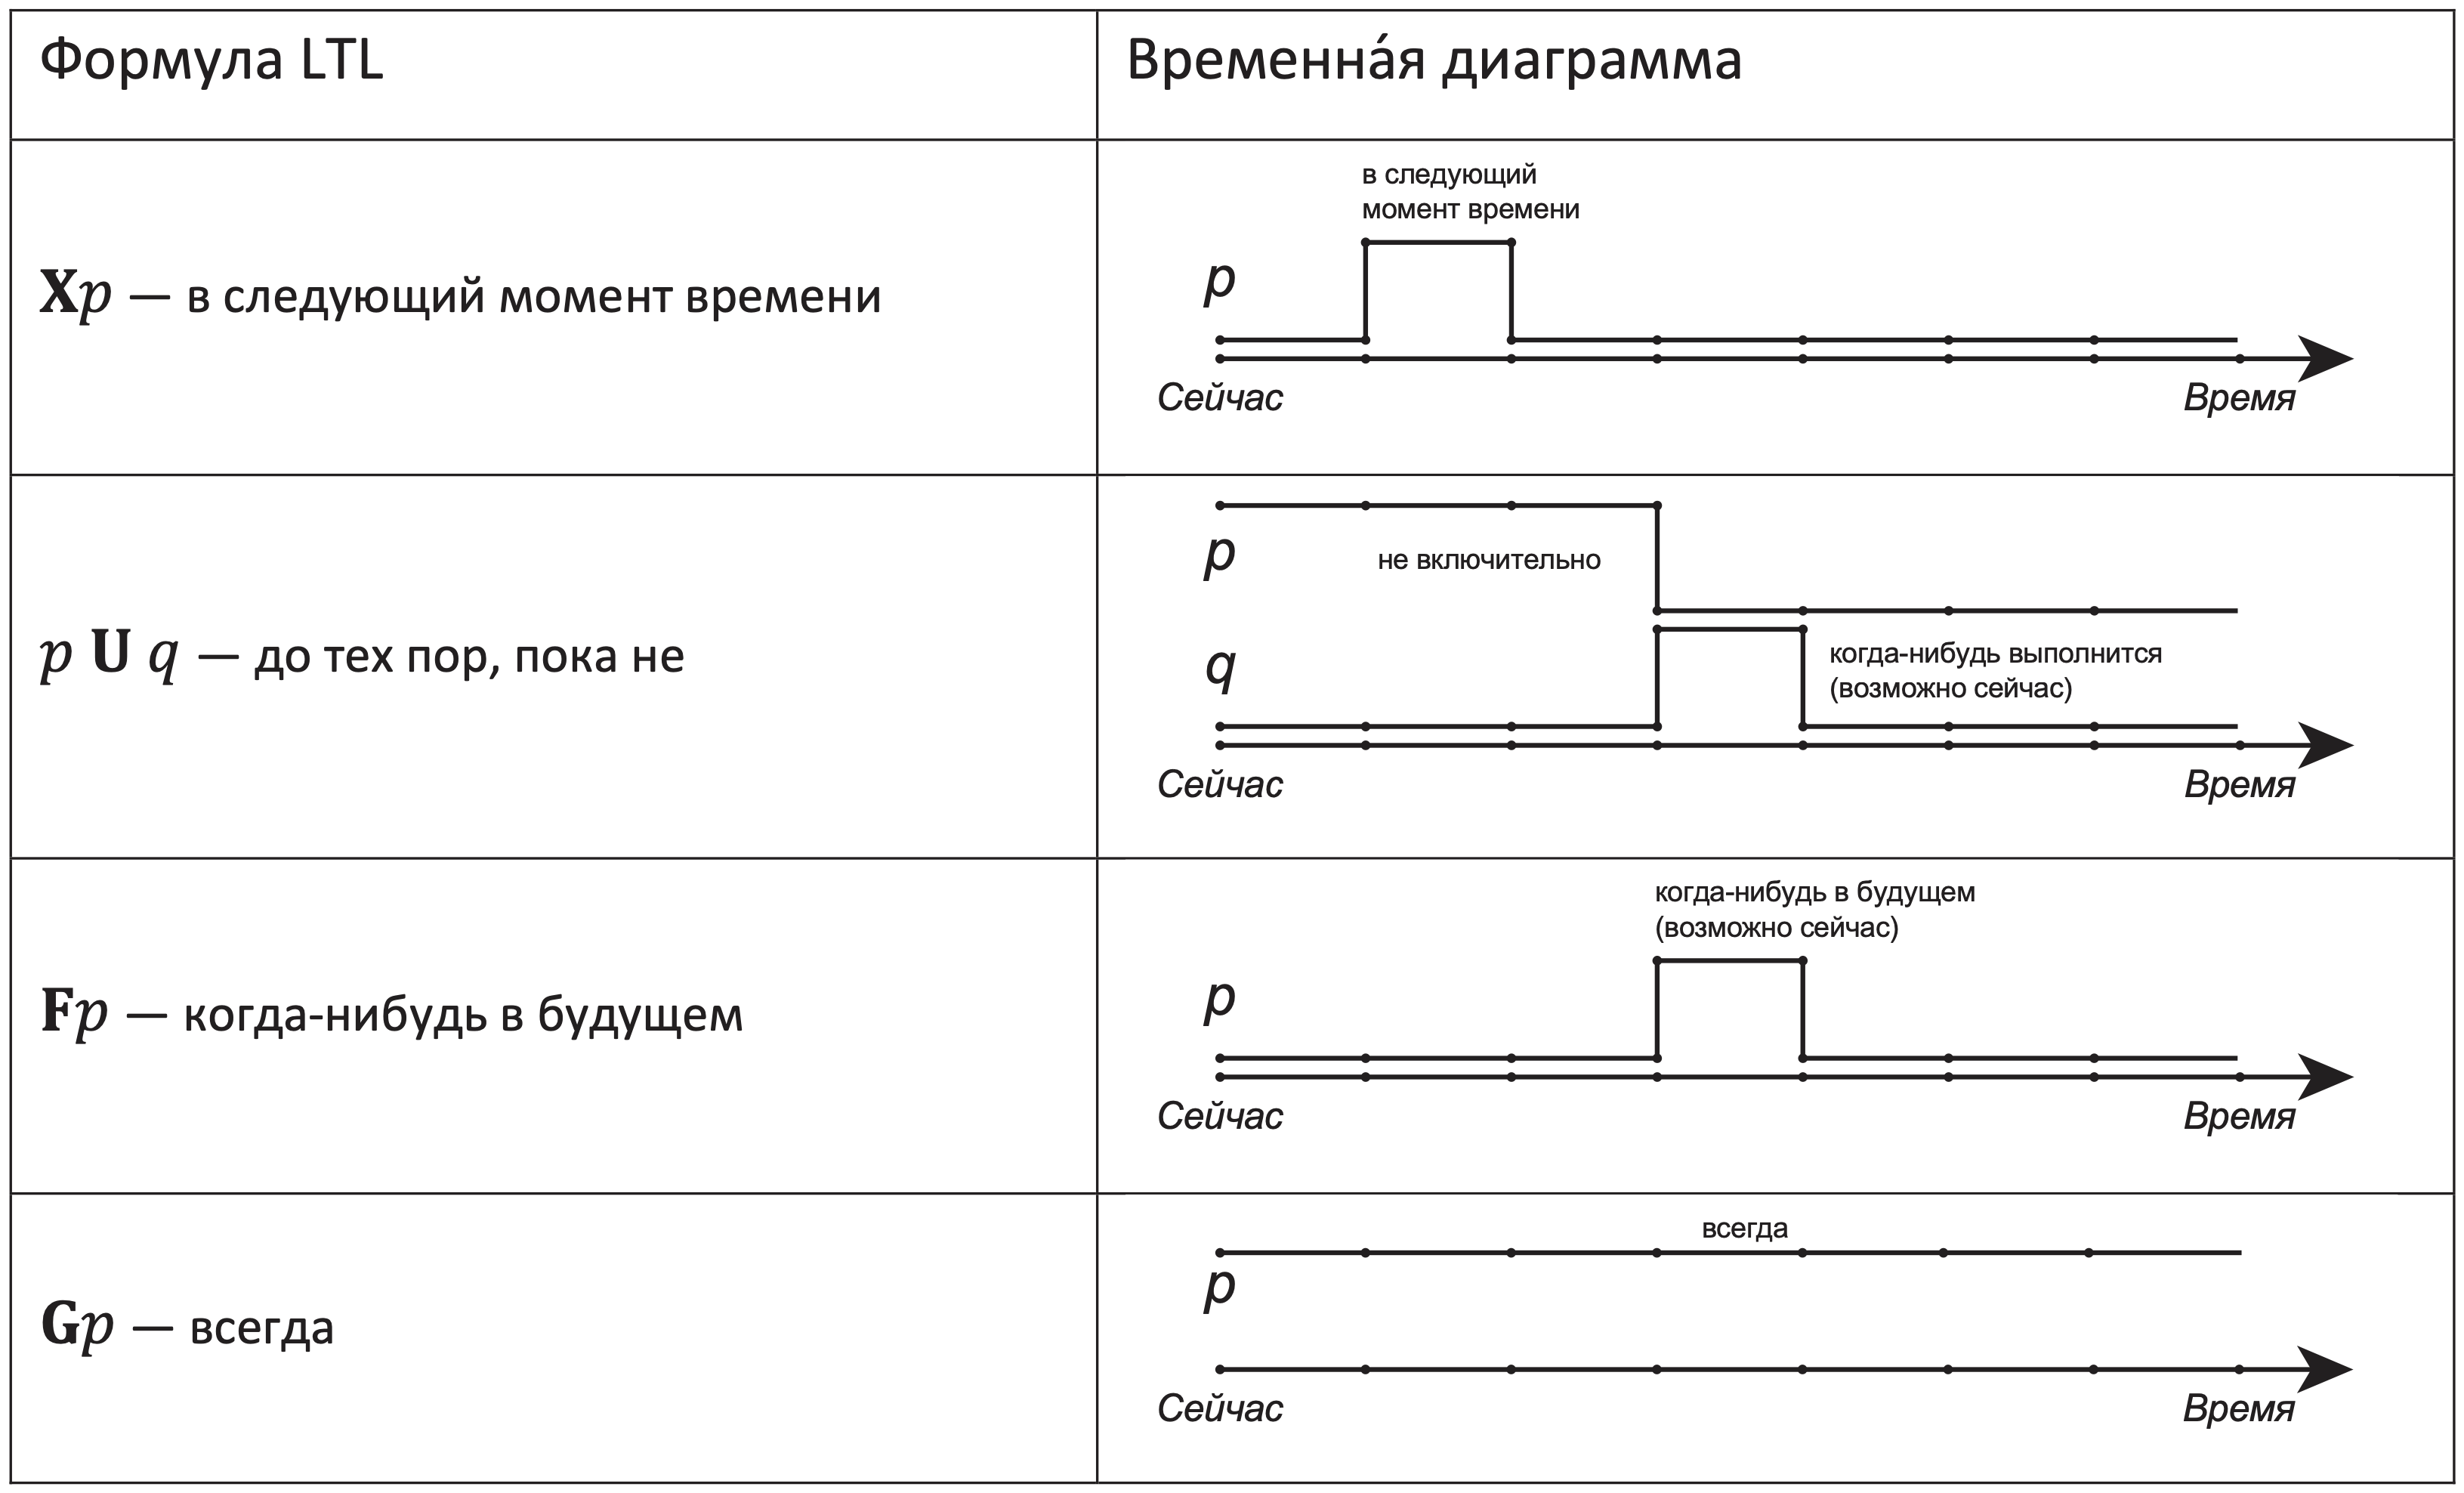
\includegraphics[width=\linewidth]{pics/ltl-timescape.png}
  \caption{LTL-futures}
  \label{LTL-futures}
\end{figure}


Параллельные программы, как и последовательные, можно верифицировать дедуктивно. 
Это справедливо как для спецификаций, заданных в форме пред- и постусловий, так и для спецификаций, выраженных на языке LTL.

Для примера обратимся к \textbf{алгоритму Петерсона} (Gary Peterson) взаимного исключения процессов. 
Пусть программа P состоит из двух процессов $P_0$ и $P_1$, работающих в бесконечном цикле. 
Периодически каждый из них входит в критическую секцию (для процесса $P_i$ критическая секция помечена меткой $CRS_i$). 
Вход процесса в критическую секцию осуществляется в два этапа: сначала он сообщает о своем намерении (метка $ SET_i$), затем ожидает возможности войти (метка $TST_i$). 
Выход процесса из критической секции осуществляется путем сброса флага $flag_i$, установленного при входе (метка $RST_i$). Описание процесса $P_i$ приведено ниже (\ref{LTL-code}):

\begin{figure}[H]
  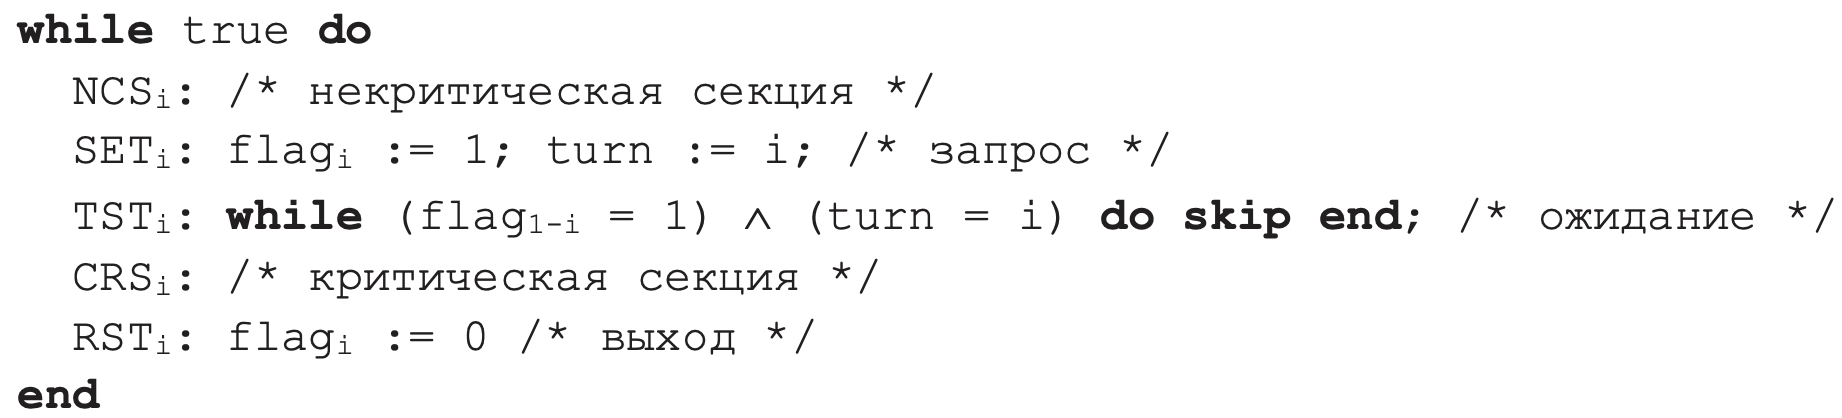
\includegraphics[width=\linewidth]{pics/ltl-sample-code.png}
  \caption{}
  \label{LTL-code}
\end{figure}

Начальное состояние задается равенствами turn = 0 и $flag_i$, где i = 0,1. Докажем корректность приведенной реализации алгоритма Петерсона относительно следующей LTL-спецификации:

\begin{itemize}
	\item $\textbf{G}\{\neg (@CRS_0 \wedge @CRS_1)\}$ -- свойство $\textit{безопасности}$ (safety): два процесса не могут одновременно пребывать в одной критической секции.
	\item $\textbf{G}\{@SET_i \rightarrow \textbf{F} @ CRS_i\}$, где $i \in \{0, 1\}$, -- свойство $\textit{живости}$ (liveness): если процесс запросил доступ к критической секции, то рано или поздно он его получит.
\end{itemize}

При этом \textit{справедливость} планировщика, о которой говорилось выше, при помощи LTL-формул задаётся вот так:

\begin{figure}[H]
  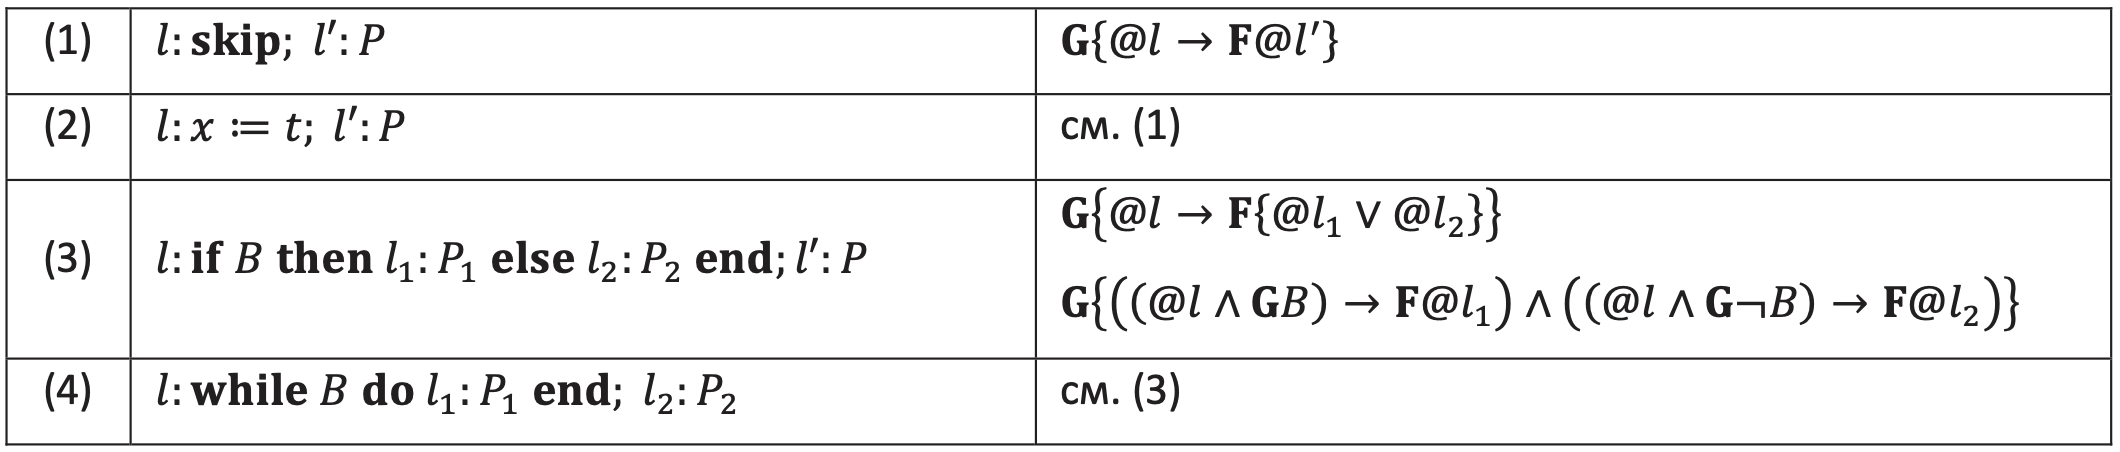
\includegraphics[width=\linewidth]{pics/ltl-scheduler.png}
  \caption{Формулы, задающие справедливость планировщика}
  \label{LTL-scheduler}
\end{figure}